 \documentclass[10pt,letterpaper]{article}
 \usepackage[left=1.8cm, right=1.8cm, top=1cm]{geometry}
 \usepackage[utf8]{inputenc}
 \usepackage[T1]{fontenc}
 \usepackage[spanish]{babel}
 \usepackage{amsmath}
 \usepackage{amsfonts}
 \usepackage{amssymb}
 \usepackage{graphicx}
 \usepackage{subfigure}
 \usepackage{steinmetz}
 \usepackage{float}

\author{Clase Práctica $\#$9}
\title{Electrónica I}
\date{Ejercicios sobre polarización de los transistores bipolares.}

\begin{document}
	\maketitle

Bibliografía: Electrónica: Teoría de Circuitos y Dispositivos Electrónicos. Robert L. Boylestad y Louis Nashelsky, 10ma ed. Capítulos 3 y 4.
\\
	
	1 - ¿Cuál es la tensión entre el emisor y la tierra en la figura? ¿Y entre el colector y el emisor?
	
%	\begin{center}
	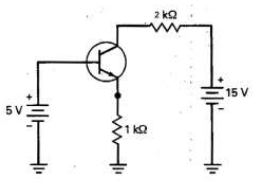
\includegraphics[scale=0.7]{c1.png} \\
%	\end{center}

	2 - Para la red de polarización de emisor de la figura, determine:
	
		a)$I_B \:$ 	b)$I_C \:$ c)$V_{CE}\:$ d)$V_{C}\:$ e)$V_{E}\:$ f)$V_{B}\:$ g)$V_{BC}\:$
		
%	\begin{center}
		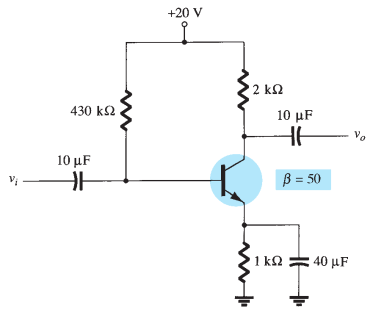
\includegraphics[scale=0.7]{c2.png}
%	\end{center}
	
	\pagebreak
	3 - Determine el voltaje de polarización $V_{CE}$ y la corriente $I_{C}$ para la configuración de polarización del divisor de voltaje de la figura:
	
%	\begin{center}
		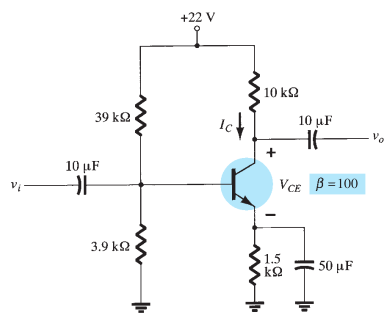
\includegraphics[scale=0.6]{c4.png} \\
%	\end{center}

	4 - Determine $V_{CE_{Q}}$ y $I_{E_{Q}}$ para la red de la figura:
		
%	\begin{center}
		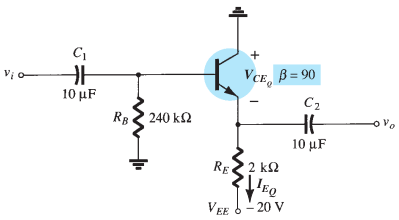
\includegraphics[scale=0.7]{c3.png} \\
%	\end{center}

	5 - Calcule la corriente constante $I$ en el circuito de la figura:
	
%	\begin{center}
		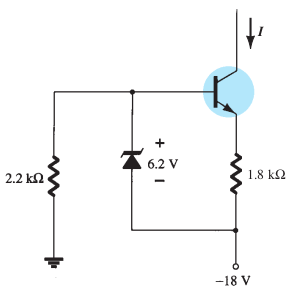
\includegraphics[scale=0.7]{c5.png}
%	\end{center}

	\pagebreak
	6 - Determine $R_B$ y $R_C$ para el inversor de transistor de la figura si $I_{C_{sat}} = 10 \mathrm{mA}$.
	
%	\begin{center}
		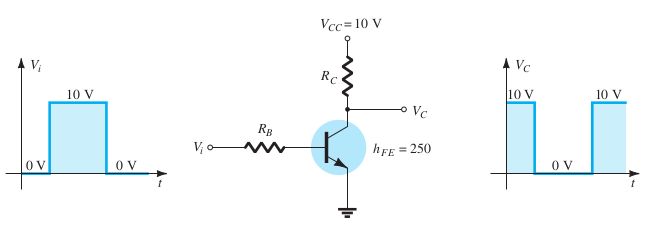
\includegraphics[scale=0.7]{c6.png} \\
%	\end{center}
	
	7- Para el amplificador de la figura determine:
	
	a) Corrientes de base y colector de cada transistor.
	
	b) Voltajes en la base, emisor y colector de cada transistor.
	
	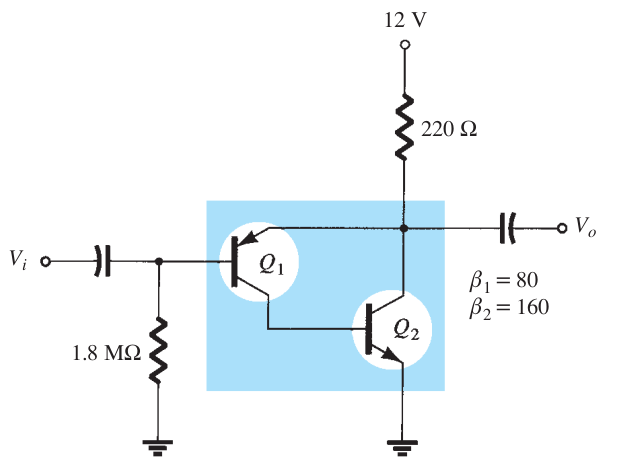
\includegraphics[scale=0.5]{c7.png}
\end{document}